\section{Mathematical Preliminaries}
\subsection{Directed Graph}
A directed graph $\mathcal{G}$, consists of a pair of finite sets, $(\emph{V},\emph{E})$. The elements of $\emph{V}$ are the vertices and the elements of $\emph{E}$ are the edges. An edge is a set formed by pairs of vertices. Further to this, there is a function, $\tau$, that associates an ordered pair of vertices for each edge in $\emph{E}$. The direction of an edge $\emph{e} = \{v_1, v_2\}$, is said to be $\tau(\emph{e}) = (v_1, v_2)$, where $\tau_{1}(e) = v_1$ is the source vertex and $\tau_{2}(e) = v_2$ is the target vertex.

With our definitions, there comes a constraint for the function $\tau$.
\begin{itemize}
\item There are no self-loops, that is for each $\emph{e} \in \emph{E}$, if $\tau(\emph{e}) = (v_1, v_2)$ then $v_1 \neq v_2$.
\end{itemize}

There may exist neurons that are reciprocally connected, that is, there may be edges whereby we have $\emph{e}, \emph{e}^\prime \in \emph{E}$ such that $\tau(\emph{e})=(v_1,v_2)$ and $\tau(\emph{e}^\prime) = (v_2,v_1)$.

A vertex $\emph{v} \in \mathcal{G}$ is said to be a sink if there exists no $\emph{e} \in \emph{E}$ such that $\emph{v}=\tau_1(\emph{e})$, but there is at least one edge $\emph{e}^\prime \in \emph{E}$ such that $\tau_2(\emph{e}^\prime) = \emph{v}$. Similarly, \emph{v} is said to be a source if there exists no $\emph{e} \in \emph{E}$ such that $\emph{v} = \tau_2(\emph{e})$, but there is at least one $\emph{e}^\prime \in \emph{E}$ such that $\tau_1(\emph{e}^\prime) = \emph{v}$.

A path in a directed graph consists of a sequence of edges $(e_1, e_2, ..., e_n)$ such that for all $1 \leq k \leq n$, the target of $e_k$ is $e_{k+1}$, i.e.~$\tau_2(\emph{e}_k) = \tau_1(\emph{e}_{k+1})$. The length of the path $(e_1, e_2, ..., e_n)$ is $n$.

If the target of $e_n$ is the source of $e_1$, that is $\tau_2(\emph{e}_n) = \tau_1(\emph{e}_1)$, then $(e_1, ..., e_n)$ is an oriented cycle. A directed graph that contains no oriented cycle is said to be acyclic.

A directed graph is said to be fully connected if for every pair of distinct vertices, there exists a path from one to the other, in at least one direction.
\subsection{Simplices}
A simplex is a generalisation of the notion of a point, a line, a triangle up to some arbitrary dimension. The simplex is named as such since it is the simplest possible polytope in any given space.

We have, for example, the following possible simplices:

\begin{itemize}
    \item A 0-simplex which consists of a vertex.
    \item A 1-simplex which consists of two vertices and an edge with direction.
    \item A 2-simplex which consists of three vertices and three edges all having direction. There is also a clear source and a clear sink. An example is given below.
    \item A 3-simplex consists of 4 vertices and 6 edges all having direction and where we have a clear source and a clear sink.
\end{itemize}
To generalise this, a $k$-simplex is the convex hull of the $k+1$ vertices it contains \cite{2018}.
\begin{figure}[H]%
    \centering
    \captionsetup{justification=centering}
    \subfloat[\centering 0 Simplex]{{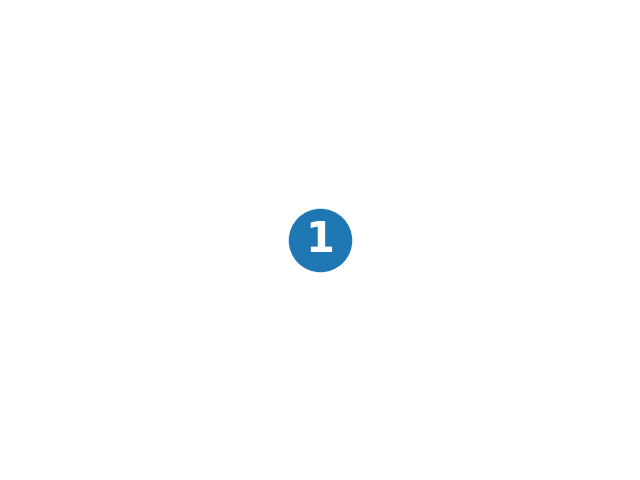
\includegraphics[width=3cm]{graph/0simplex.png} }}%
    \qquad
    \subfloat[\centering 1 Simplex]{{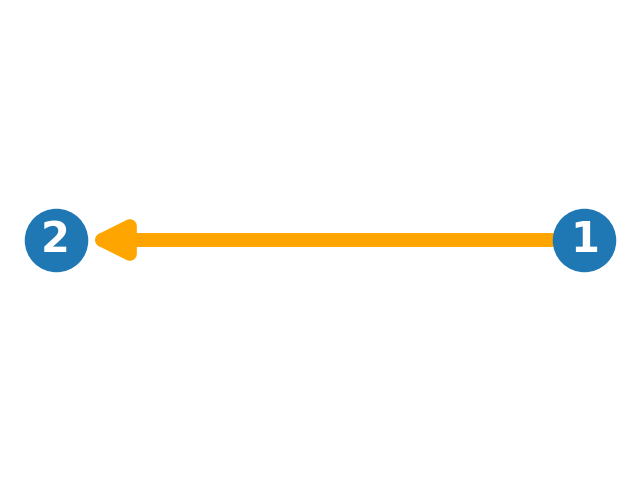
\includegraphics[width=3cm]{graph/1simplex.png} }}%
    \qquad
    \subfloat[\centering 2 Simplex]{{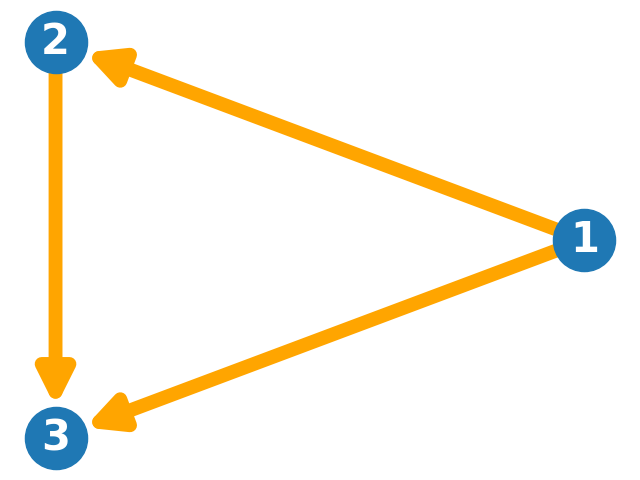
\includegraphics[width=3cm]{graph/2simplex.png} }}%
    \qquad
    \subfloat[\centering 3 Simplex]{{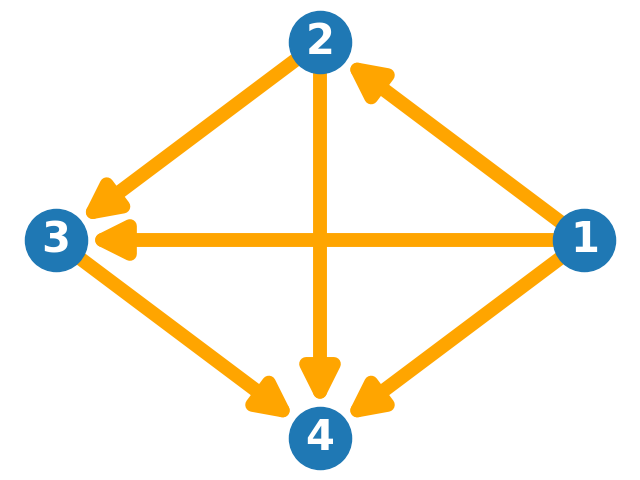
\includegraphics[width=3cm]{graph/3simplex.png} }}%
    \caption{Simplices from dimension 0 through to 3}%
    \label{fig:example}%
\end{figure}

\subsection{Simplicial Complex}
An abstract simplicial complex $\emph{S}$, is a collection of finite sets. These sets are closed under taking subsets, that is, every subset of a set in the family is also in the family. As an example, in a 2 dimensional simplicial complex, we have triangles, which are sets of size 3, their edges, which are sets of size 2 and their vertices which are sets of size 1 \cite{2008Gregarxiv:0809.4221}.

However, we have a slight variation on this in that we have an abstract $\emph{directed}$ simplicial complex. This is where we again have a collection of sets denoted $\emph{S}$. However, this time, the sets are finite and ordered with the property that if $\sigma \in \emph{S}$, then every subset $\tau$ of $\sigma$, with the natural ordering inherited from $\sigma$, is also a member of $\emph{S}$.

The elements $\sigma$ of a simplicial complex $\emph{S}$, are simplices. We define the dimensionality of $\sigma$ to be the cardinality of the set minus one. Therefore, if $\sigma$ is a simplex of dimension $n$, then we refer to $\sigma$ as an $n$-simplex of $\emph{S}$. The set of all simplices of $\emph{S}$ is denoted $\emph{S}_n$. A simplex $\tau$ is said to be a face of $\sigma$ if $\tau$ is a subset of $\sigma$ with a strictly smaller cardinality than $\sigma$. As an example, let's take Figure 3(c). This shows a simplex $\sigma$ of dimension 2, however, we can also consider the edge from vertex 1 to vertex 3 as a face of the 2 dimensional simplex, since this is defined using $\tau$(e) = ($v_1, v_3$) where $\tau$ is a subset of $\sigma$.

These simplices may be joined along these faces. A simplex that is not the face of any other simplex is said to be maximal. Again, with the 2-simplex above, we can see that the maximal dimension of this is 2, and that the edges and vertices that construct this object are faces of the 2-simplex and faces of faces of the 2-simplex respectively. Thus, the set of all maximal simplices of a simplicial complex determines the entire simplicial complex since this is made up entirely of maximal simplicial complexes or a face of a simplicial complex.

\subsection{Simplicial Complex applied to Directed Graphs}
The directed graph $\mathcal{G}$ naturally creates the directed simplicial complex. The directed simplicial complex that is associated to the directed graph $\mathcal{G}$ is called the directed flag complex of $\mathcal{G}$.

The directed flag complex is defined to be the ordered simplicial complex whose $n$-simplices are all ordered $(n+1)$-cliques. So, let it be that $\sigma = (v_0, v_1, ...v_n)$, such that $v_i \in \emph{V}$ for all $i$ and ($v_i, v_j) \in \emph{E}$ for $i < j$. Then the ordered set of these completes the directed flag complex. Further to this, we note that $v_0$ is the initial vertex, or the source of $\sigma$, and that $v_n$ is the final or sink of $\sigma$.

One final thing of note is that because of our assumption on $\tau$, an $n$-simplex in $\emph{S}$ is characterised by the ordered sequence $(v_o, v_1, ..., v_n)$ and not by the vertices. By example, $(v_0, v_1, v_2)$ and $(v_0, v_2, v_1)$ are two distinct 2-simplices that contain the same set of vertices.

\subsection{Directionality}
The directionality \cite{Reimann_2017} of a directed graph $\mathcal{G}$ is given by:
\begin{equation}
    \Dr(\mathcal{G}) = \sum_{v \in V} \sd(\emph{v})^2 \enspace{,}
\end{equation}
where
\begin{equation}
    \sd(\emph{v}) = \Indeg(\emph{v}) - \outd(\emph{v})\enspace{.}
\end{equation}
The signed degree ($\sd$) is given as the in-degree minus the out-degree for each vertex in $\mathcal{G}$. That is, the number of times a given vertex is a target vertex minus the number of times the same given vertex is a source vertex. Following on from this, the directionality of $\mathcal{G}$ is the sum of the squares of all the signed degrees for each vertex in the directed graph $\mathcal{G}$.

Further to this, we can note that the sum of the signed degree for a finite graph is zero. That is,
\begin{equation}
    \sum_{v \in \mathcal{G}}\sd(\emph{v}) = 0 \enspace{.}
\end{equation}

\subsection{Homology}
Simplicial homology arose as a way to study topological spaces. The building blocks of which are our $n$-simplices. On top of this, we have further numerical quantities in order to describe the abstract directed flag complex. These include Betti numbers and the Euler Characteristic. These are described below.

\subsection{Betti Numbers}
Informally, the $k^{th}$ Betti number refers to the number of $k$-dimensional holes on a topological space, where a $k$-dimensional hole is a $k$-dimensional cycle that is not a boundary of a $(k+1)$-dimensional object.

The definitions of the first few Betti numbers are as follows;
\begin{itemize}
    \item $\beta_0$ is the number of connected components
    \item $\beta_1$ is the number of 1-dimensional or `circular' holes.
    \item $\beta_2$ is the number of 2-dimensional `voids' or `cavities'.
\end{itemize}
For example, let's take our triangular prism in Figure 4. We can see that the vertices are all connected as one object. This, as well as with the Bio-M MC, takes the zeroth Betti number to be 1. That is, $\beta_0 = 1$. Next, we take the informal definition of the 1-dimensional Betti number. We can see here that there are no holes that are of dimension 1, so $\beta_1 = 0$. Finally, we look at the second dimensional definition of a Betti number. We are looking for holes or cavities that are entirely enclosed by 2-dimensional objects. We can see that we have a hole that is enclosed by triangles. Therefore, $\beta_2 = 1$. Applying the Euler Characteristic to the Betti numbers of this example, we have,
\begin{equation}
    \beta_0 - \beta_1 + \beta_2 = 1 - 0 + 1 = 2
\end{equation}
So if we take the classical usage of the Euler characteristic, we can see the relationship, as stated above in the Euler characteristic section, is also 2 as follows:
\begin{equation}
    V - E + F = 6 - 8 + 12 = 2
\end{equation}

\begin{figure}[H]%
    \centering
    \captionsetup{justification=centering}
{{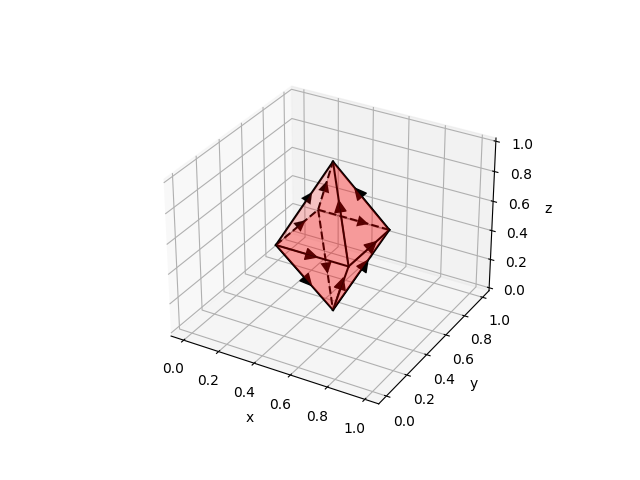
\includegraphics[width=12cm]{graph/simplex_structure.png} }}%
    \caption{Triangular Prism}
    \label{fig:example}%
\end{figure}

Now, informally, let $\mathbb{F}_2$ denote a field of two elements. Let $\emph{S}$ be a simplicial complex. Define the chain complex C*(S, $\mathbb{F}_2$) to be the sequence ($C_n$ = $C_n$(S,$\mathbb{F}_2$))$_{n\geq0}$, such that $C_n$ is the $\mathbb{F}_2$-vector space whose basis elements are the $n$-simplices $\sigma \in  S_n$, for each $n\geq0$. In other words, the elements of $C_n$ are formal sums of $n$-simplices in S.

For each $n\geq1$, there is a linear transformation called a \textit{differential}
\begin{equation}
    \partial_n : C_n \rightarrow C_{n-1} \enspace{.}
\end{equation}
specified by $\partial_n(\sigma) = \sigma^0 + \sigma^1 + ... + \sigma^n$ for every $n$-simplex $\sigma$, where $\sigma^i$ is the $i^{th}$ face of $\sigma$. Having defined $\partial_n$ on the basis, one then extends it linearly to the entire vector space $C_n$. The $n^{th}$ Betti number $\beta_n$(S) of a simplicial complex $\emph{S}$ is the $\mathbb{F}_2$-vector space dimension of its $n^{th}$ mod-2 homology group, which is defined by,
\begin{equation}
    \mathbb{H}_n(\emph{S}, \mathbb{F}_2) = \frac{\Ker(\partial_n)}{ \ime(\partial_{n+1})} \enspace{,}
\end{equation}
for  $n\geq 1$ and
\begin{equation}
    \mathbb{H}_0(\emph{S}, \mathbb{F}_2) = C_0/\ime(\partial_{1}) \enspace{.}
\end{equation}
For all $n\geq1$, there is an inclusion of vector subspaces i.e.~$\ime(\partial_{n+1}) \subseteq \Ker(\partial_{n}) \subseteq C_n$, and thus the definition of homology makes sense.

Computing Betti numbers of a simplicial complex is conceptually very easy. Let $|S_n|$ denote the number of $n$-simplices in the simplicial complex $\emph{S}$. If one encodes the differential $\partial_{n}$ as a $(|\emph{S}_n-1| \times |\emph{S}_n|)$-matrix $D_n$ with entries in $\mathbb{F}_2$, then one can easily compute its \textit{nullity}, null($\partial_n$), and its rank, rk($\partial_n$), which are the $\mathbb{F}_2$ dimensions of the null-space and the column space of $D_n$ respectively. The Betti numbers of $\emph{S}$ are then a sequence of natural numbers defined by,
\begin{equation}
    \beta_0(\emph{S}) = \text{dim}_{\mathbb{F}_2}(C_0) - \text{rk}(\partial_1) \enspace{,}
\end{equation}
\begin{equation}
    \beta_{n}(\emph{S}) = \text{null}(\partial_{n}) - \text{rk}(\partial_{n+1}) \enspace{.}
\end{equation}

Since Im($\partial_{n+1}$) $\subseteq$ Ker($\partial_n$) for all $n\geq 1$, the Betti numbers are always non negative. The $n^{th}$ Betti number $\beta_n$ gives an indication of the n-dimensional cavities in the geometric realisation of S \cite{Reimann_2017}.

\subsection{Euler Characteristic}
The Euler Characteristic is simply defined as the alternating sum of the number of simplices in each dimension. This can also be applied to Betti numbers in each dimension, however, for the Betti numbers for our models and even the \ER model in dimensions 1 through 3, this is not computationally viable since the required memory to compute the Betti numbers in these dimensions is upwards of 16GB.

So, algebraically, the Euler Characteristic is given as follows:
\begin{equation*}
    \chi = k_0 - k_1 + k_2 - k_3 + ...
\end{equation*}
\begin{equation}
    \Rightarrow \chi = \sum_{k \geq 0} (-1)^k \abs{S_k} \enspace{.}
\end{equation}
As a side note, there is a close relationship between the Euler Characteristic and Betti numbers \cite{Reimann_2017}. This relationship is as follows:
\begin{equation}
    \chi(\emph{S}) = \sum_{k\geq 0}(-1)^k \beta_{k}(\emph{S})
\end{equation}


\subsection{Blocks}
Within the MC we have a set of neurons and a set of synapses, represented by vertices and directed edges respectively. Now, when we take into account the direction of information flow, an edge has with it a pair of ordered vertices.

Now, when we subdivide the MC on a layer by layer basis, we are left with 25 subsets of ordered pairs of vertices, each belonging to a ``block''. An example of a block is L1-L4. That is, we have a set of ordered vertices where the pre-synaptic neurons set is from Layer 1 and the post-synaptic neurons are from Layer 4.

This is not to say that there are a specific set of neurons that are pre-synaptic or post-synaptic, but rather, the neuron's state is determined by the order in which it appears in the ordered pair $\emph{e}$.


\subsection{Total Variation distance}
Here, we use the Total Variation (TV) distance to quantify statistical differences between distributions obtained from our models.

Let $f$ and $g$ be two discrete distributions over a common support set $\{1,2,\ldots,n\}$.
Thus, $\sum_{i=1}^{n}f_{i} = 1$ and $\sum_{i=1}^{n}g_{i} = 1$.

Typically, we want to compare distribution $f$ obtained from a model with the distribution $g$ obtained from the Bio-M MC. To compare the distance between these two distributions, we take:
\begin{equation}
\delta(f, g) = \sum_{i=1}^{n}(|f_{i} - g_{i}|)\enspace{.}
\end{equation}

This will output a value in the range $[0, 2]$.
Clearly $\delta(f, g)=0$ if $f=g$ and $\delta(f, g)=2$ if $f$ and $g$ have no common events.
